\documentclass[conference]{IEEEtran}
\usepackage[T1]{fontenc}
\usepackage{amsmath,amssymb}
\usepackage{graphicx}
\usepackage{booktabs}
\usepackage{cite}
\usepackage[hidelinks]{hyperref}

\graphicspath{{figures/}}

% Numbers are from robotnik_arm/experiments/ablation/results/rel_study/.
% Figures: robotnik_arm/experiments/ablation/report_figures.py writes figures/*.pdf
% from saved results; report_rollouts.py and report_dart_stats.py produce the
% per-episode inputs that three_models.json did not keep.
% Budget: six IEEE pages including references; the contribution statement
% may occupy a separate seventh page.

\title{Learning to Catch with Behaviour Cloning:\\
Accuracy and Closed-Loop Failure Analysis}
\author{\IEEEauthorblockN{William Boyd, Nick Wright, Yiyan Wang}
\IEEEauthorblockA{University College London\\London, United Kingdom}}

\begin{document}
\maketitle

\begin{abstract}
A flat behaviour-cloning policy imitates a scripted controller that intercepts a ball with a mobile manipulator. Before any sweep, we diagnose a $10\,\mathrm{Hz}$ baseline: its arm catches when the expert has parked the base, but its own driving leaves the base off target, and the expert's wheel command changes substantially within one $100\,\mathrm{ms}$ hold. A pre-registered sweep of policy rate, history, prediction horizon and execution window then selects $25\,\mathrm{Hz}$, predicting $2\,\mathrm{s}$ and executing $1\,\mathrm{s}$, with no history. It halves the mean miss, from $113$ to $59\,\mathrm{mm}$, and raises the share of episodes within $10\,\mathrm{mm}$ from $0.7\%$ to $3.2\%$. It does so by parking the base twice as close to the expert's point; at equal parking error the two policies miss by the same amount. In both, sideways parking error alone explains over $80\%$ of the mean squared miss, because the hand does not correct it. Retraining on high-amplitude DART noise matched to the winner's own command error makes the policy worse ($90\,\mathrm{mm}$), because noise of that size drives the expert's base a median $1.2\,\mathrm{m}$ off its route and the expert catches none of those demonstrations. Retraining instead on demonstrations that park the base off the expert's point lowers the miss to $28\,\mathrm{mm}$, with $91\%$ of episodes within $50\,\mathrm{mm}$, by teaching the arm to absorb sideways parking error. Along-track parking error is the largest attributable part of what remains.
\end{abstract}

\begin{IEEEkeywords}
Imitation learning, mobile manipulation, robotic catching, evaluation
\end{IEEEkeywords}

\section{Introduction}
\subsection{Problem and Scope}
We extend a fixed-target reaching task to moving-target interception (``ball catching'') with a mobile base and a seven-joint arm. A neural network is trained by behaviour cloning to imitate the commands of an expert controller~\cite{pomerleau1991}. To catch a moving ball the robot can meet it at many points along its path, so the problem changes from reaching one fixed target to choosing among several valid interceptions.

A model may match the expert's recorded commands closely and still miss the ball, because each small mistake moves the robot into states the expert never visited and changes every command that follows~\cite{ross2011}. We therefore evaluate in closed loop: the learner drives the simulated robot from its initial state until a catch or timeout, and we measure the hand-to-ball distance together with the base position that produced it. Inputs are simulated state, ball paths are ones the expert can catch, and a catch is the hand coming within a set distance of the ball, without a grasp.

\subsection{Research Question and Contributions}
We ask how policy rate, observation history, prediction horizon and execution window affect catching accuracy, and what limits the best configuration. The contributions are:
\begin{itemize}
\item a pre-registered diagnosis of the $10\,\mathrm{Hz}$ baseline that locates its error in base driving rather than the arm, and predicts which factors should help (Fig.~\ref{fig:baseline});
\item a one-factor sweep and combination stage that halves the mean miss by raising the policy rate to $25\,\mathrm{Hz}$ (Figs.~\ref{fig:sweep}--\ref{fig:progression});
\item a matched comparison of two ways of enlarging the demonstrations: high-amplitude DART command noise~\cite{laskey2017}, which fails, and deliberate parking offsets, which lower the miss to $28\,\mathrm{mm}$ (Figs.~\ref{fig:dart}--\ref{fig:remaining}).
\end{itemize}
Unsuccessful episodes are kept throughout, so the analysis can show where the error remains.

\section{Methodology}
\subsection{Simulation Environment and Task Definition}
The simulated robot has a skid-steer base, a seven-degree-of-freedom Kinova arm and a passive hand. PyBullet provides the physics~\cite{pybullet} and Pinocchio the kinematics and rigid-body dynamics~\cite{pinocchio}. The simulation advances in $1\,\mathrm{ms}$ steps within a workspace of $5\times5\,\mathrm{m}$ horizontally, centred on the robot's initial base position, with height limits of $0.07$--$1.30\,\mathrm{m}$ (Fig.~\ref{fig:task}). Each ball follows a seeded parabola between randomly sampled points on opposite vertical faces of the workspace. Its apex is sampled between $0.5$ and $1.5\,\mathrm{m}$ above the roof, so the ball leaves the workspace and re-enters before reaching the opposite face. A path is kept only if the expert planner finds a feasible interception before the endpoint.

\begin{figure}[t]
\centering
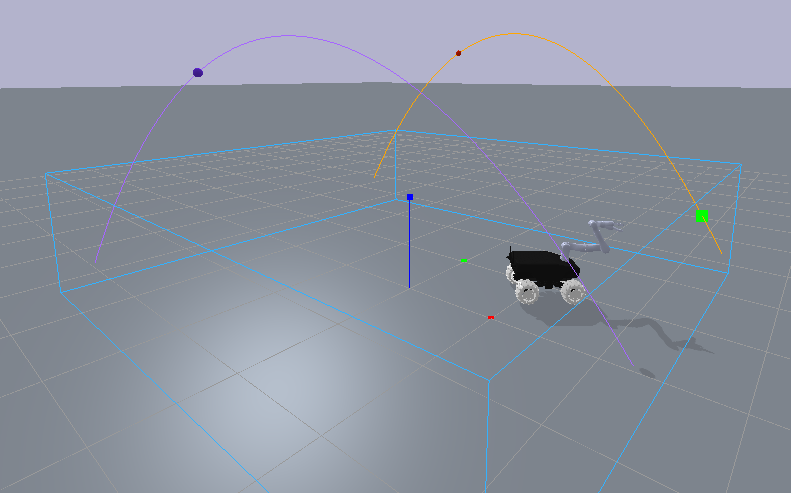
\includegraphics[width=0.8\columnwidth]{image.png}
\caption{Simulated single-ball catching task, showing the mobile robot, the workspace boundaries and the target interception point.}
\label{fig:task}
\end{figure}

\subsection{Expert and Demonstration Generation}
We extend the provided fixed-target expert with an interception planner that estimates the ball's velocity and acceleration from three position observations. It searches future points along the predicted path in $0.1\,\mathrm{s}$ increments and selects the earliest feasible interception after re-entry, together with a base position and heading from which the arm can reach it. Feasibility accounts for base travel, turning and arm motion, with extra time for settling. The existing base and arm controllers then move towards these goals, replanning if the interception is missed by more than $1\,\mathrm{s}$. The network is trained to predict the wheel and arm commands this expert produces.

\subsection{Datasets}
The baseline and the factor sweep use 1,000 demonstrations, one per training scene, resampled to a $50\,\mathrm{Hz}$ grid. Odd-indexed demonstrations already carry a small perturbation added at collection~\cite{laskey2017}: Gaussian noise on the applied wheel and arm torques, with standard deviations $0.08$ and $0.2\,\mathrm{N{\cdot}m}$, clipped at three standard deviations and held for $50\,\mathrm{ms}$, with the clean expert command stored as the label. Master seed 2026 generates the 1,000 training scene seeds and 200 separate evaluation scene seeds from the same distributions.

After a winner is selected, it is retrained on two extended sets (Table~\ref{tab:datasets}). Each adds 1,000 episodes on the training seeds. The \emph{command-noise} set executes the expert under high-amplitude noise matched to the winner's own command error (Section~\ref{sec:dart}) and stores the clean expert command as the label. The \emph{parking-offset} set shifts the expert's parking goal and leaves the commands clean: shifts along and across the route are drawn from zero-mean Gaussians with standard deviations $20$ and $50\,\mathrm{mm}$, and the shift is capped at $150\,\mathrm{mm}$. The two extensions add the same scenes and the same number of episodes, and differ only in what is perturbed.

\begin{table}[t]
\centering
\caption{Demonstration sets. The extensions reuse the training scene seeds.}
\label{tab:datasets}
\footnotesize
\begin{tabular}{lcl}
\toprule
Set & Episodes & What is added \\
\midrule
Ablation & 1,000 & Low-amplitude torque noise on odd episodes \\
Command noise & 2,000 & 1,000 high-amplitude DART episodes \\
Parking offset & 2,000 & 1,000 shifted parking goals \\
\bottomrule
\end{tabular}
\end{table}

\subsection{Observation Representation and Temporal Context}
Each raw observation has 42 values: time; ball position, velocity and acceleration; base position; heading as sine and cosine; base linear and angular velocity; seven arm joint positions and velocities; four wheel velocities; and end-effector position. Ball velocity and acceleration are estimated from the last three $1\,\mathrm{ms}$ samples, as the expert does. Every model, including the baseline, appends twelve base-frame features: the ball position relative to the base origin, and the ball velocity, ball acceleration and ball-to-hand displacement rotated into the robot's forward, sideways and vertical axes. The baseline sees the current frame only; history is a swept factor.

\subsection{Policy Architecture and Action Chunking}
The network is a multilayer perceptron with three hidden layers of width 512 and ReLU activations, followed by a linear head. Without history the input is the current 54-value frame; a stack flattens several frames, and the GRU variant (hidden size 128) appends its final state to the current frame. The head emits a chunk of 18-value commands, one per future step: four wheel velocities, seven arm joint references and seven joint-velocity references. Joint references are labelled relative to the arm position at the query and added back to that position at execution.

The simulation keeps its $1\,\mathrm{ms}$ step, and between policy queries the low-level loop holds the latest command. Wheel torque is $-30$ times the wheel-speed error; the arm uses the expert's gravity-compensated proportional-derivative law with the joint reference clipped to a limited lead from the measured angle. When the policy rate changes, predicted and executed durations stay fixed in seconds, so a faster policy predicts more steps.

\subsection{Training Configuration}
Inputs are standardised with training-set statistics and action targets with statistics from up to 50,000 sampled windows; standard deviations are floored at $10^{-3}$ and normalised inputs clipped to $[-10,10]$. The loss is the mean squared error over the normalised action chunk. Training uses AdamW (learning rate $10^{-3}$, weight decay $10^{-4}$), batch size 1,024 and 20,000 steps, with a 500-step linear warm-up followed by cosine decay to $1\%$ of the peak. There is no validation split or early stopping. Every configuration is trained with three seeds.

The baseline runs at $10\,\mathrm{Hz}$, predicts $2\,\mathrm{s}$, executes $1\,\mathrm{s}$ and uses the current frame. Rate, history and timing are changed one at a time (Table~\ref{tab:factors}) and scored as three families. A combination stage crosses the top two levels of the families that beat the baseline and adds one cell with every family that moved at its best level. A configuration ranks higher if its mean catch rate at $10\,\mathrm{mm}$ is higher; if the seed intervals overlap, the lower mean miss ranks higher.

\begin{table}[t]
\centering
\caption{One-factor levels. Unlisted settings stay at the baseline: $10\,\mathrm{Hz}$, predict $2\,\mathrm{s}$, execute $1\,\mathrm{s}$, current frame only.}
\label{tab:factors}
\footnotesize
\begin{tabular}{lp{5.2cm}}
\toprule
Factor & Levels other than the baseline \\
\midrule
Policy rate & 5, 25 and $50\,\mathrm{Hz}$ \\
History & Stacks of $0.5\,\mathrm{s}$ and $2\,\mathrm{s}$; GRU over $2\,\mathrm{s}$ \\
Prediction horizon & $1\,\mathrm{s}$ and $5\,\mathrm{s}$, execution held at $1\,\mathrm{s}$ \\
Execution window & $0.5\,\mathrm{s}$, prediction held at $2\,\mathrm{s}$ \\
Short chunk & Predict $0.5\,\mathrm{s}$; execute $0.3\,\mathrm{s}$ or $0.1\,\mathrm{s}$ \\
\bottomrule
\end{tabular}
\end{table}

\section{Evaluation Protocol}
\label{sec:eval}
\subsection{Closed-Loop Episodes and Capture Conditions}
Each model drives the simulated robot from its initial state on the same 200 evaluation scenes, so all models face the same ball paths. Distance counts only while the ball is inside the workspace after having left it. Denoting those times by $\mathcal{V}_i$, the miss in episode $i$ is
\begin{equation}
 d_i=\min_{t\in\mathcal{V}_i}\|\mathbf{p}_{\mathrm{EE},i}(t)-\mathbf{p}_{\mathrm{ball},i}(t)\|_2 .
\end{equation}
The episode ends $0.1\,\mathrm{s}$ after the hand first comes within $10\,\mathrm{mm}$ of the ball, or $1\,\mathrm{s}$ after the trajectory's end. The fingers stay at a fixed angle, so a catch is not a grasp. Every episode in this study produced a finite miss. The 200 scenes are the development benchmark used for ranking, not a final test held out from every design choice.

\subsection{Accuracy and Statistical Uncertainty}
The catch rate on $N$ scenes is $\hat{c}=\frac{1}{N}\sum_{i}\mathbf{1}\{d_i<10\,\mathrm{mm}\}$. Tables give the mean over the three training seeds with the sample standard deviation ($n-1$); medians and distributions pool the 600 episodes. Because all models face the same scenes, differences are paired, but we do not report a per-scene significance test.

\subsection{Parking Diagnostics}
At the closest approach we express the base position and the hand-to-ball vector in the expert's route frame, against the expert's base at the same time. Along one axis let $b$ be the base offset and $m$ the hand miss. The \emph{correction coefficient} is $1-s$, where $s$ is the least-squares slope of $m$ on $b$: a value of one means the arm fully absorbs the parking error, zero means the error passes straight to the hand, and a negative value means the hand error grows faster than the parking error. The expert trajectories used here are offline annotations of the same scenes, not a controller that takes over. Rollouts use the NumPy export of each checkpoint.

\section{Results and Failure Analysis}
\subsection{Why the Baseline Fails}
The measurements in Fig.~\ref{fig:baseline} were recorded on the seed-1 baseline, with thresholds fixed, before the sweep started.

\begin{figure*}[t]
\centering
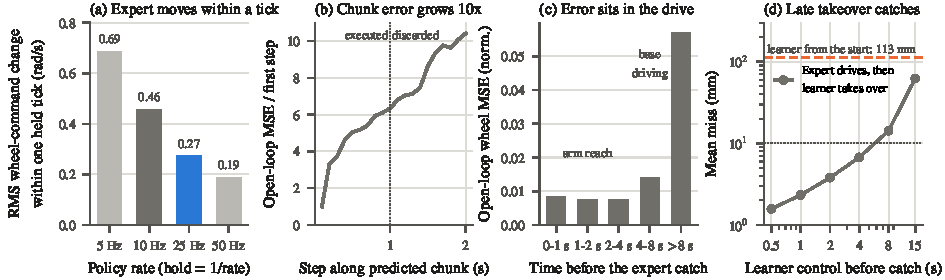
\includegraphics[width=\textwidth]{fig_baseline_diagnosis}
\caption{Pre-registered diagnosis of the $10\,\mathrm{Hz}$ baseline. (a) RMS change of the expert's wheel command within one held policy tick, over 100 demonstrations; the baseline holds each command for $100\,\mathrm{ms}$ while the expert's command moves by $0.46\,\mathrm{rad/s}$. (b) Open-loop error along the predicted $2\,\mathrm{s}$ chunk on the evaluation scenes, relative to the first step. (c) Open-loop wheel error by time before the expert's catch: it is seven times larger during the long base drive than in the last $4\,\mathrm{s}$. (d) Hand-off probe on 50 scenes: the expert drives, then the learner takes over a given time before the catch. With the base parked by the expert the learner's arm misses by $2\,\mathrm{mm}$; the miss only approaches the closed-loop value (dashed) when the learner does the driving.}
\label{fig:baseline}
\end{figure*}

The probe in Fig.~\ref{fig:baseline}(d) separates the two halves of the task. If the expert drives and the learner takes over $0.5\,\mathrm{s}$ before the catch, the mean miss is $1.6\,\mathrm{mm}$ and every episode is caught; with $1\,\mathrm{s}$, $2\,\mathrm{s}$ and $4\,\mathrm{s}$ of learner control it is $2.3$, $3.8$ and $6.7\,\mathrm{mm}$. Only when the learner controls the last $15\,\mathrm{s}$, which includes the drive, does it rise to $62\,\mathrm{mm}$, against $113\,\mathrm{mm}$ from the start of the episode. The arm has learned to reach; the error enters while the base drives and parks. Fig.~\ref{fig:baseline}(c) agrees: open-loop wheel error more than $8\,\mathrm{s}$ before the catch is $0.057$, against $0.008$ in the final $4\,\mathrm{s}$.

That error has a cause the baseline's rate makes worse. The expert's wheel command changes by $0.46\,\mathrm{rad/s}$ RMS within $100\,\mathrm{ms}$ but by $0.19\,\mathrm{rad/s}$ within $20\,\mathrm{ms}$ (Fig.~\ref{fig:baseline}(a)). A ratio of $2.42$ exceeds the pre-registered $1.5$, so a faster rate was predicted to lower the miss. The other probes gave three further predictions. Open-loop error grows $10.4$-fold along the chunk (Fig.~\ref{fig:baseline}(b)), above a threshold of $2$, predicting that a $1\,\mathrm{s}$ prediction would beat a $5\,\mathrm{s}$ one. The expert's wheel command changes $4.15$ times more over $0.5\,\mathrm{s}$ than over $0.1\,\mathrm{s}$, predicting that a $0.5\,\mathrm{s}$ chunk would increase the miss. Turning error was $0.82$ times driving error, below the threshold of $2$, so history was not indicated, and the hand-off ratio between $1\,\mathrm{s}$ and $0.5\,\mathrm{s}$ was $1.48$, below $1.5$, so a shorter execution window was not indicated either.

\subsection{One-Factor Sweep and Combination}
Table~\ref{tab:sweep} and Fig.~\ref{fig:sweep} report every level.

\begin{table}[t]
\centering
\caption{Closed-loop results on the 200 evaluation scenes: mean and sample s.d. over three seeds. The first block changes one factor; the second is the combination stage.}
\label{tab:sweep}
\footnotesize
\begin{tabular}{lcc}
\toprule
Configuration & Catch (\%) & Miss (mm) \\
\midrule
$10\,\mathrm{Hz}$ baseline & $0.7\pm 0.3$ & $113.3\pm 2.8$ \\
$5\,\mathrm{Hz}$ & $0.2\pm 0.3$ & $229.5\pm 5.5$ \\
$25\,\mathrm{Hz}$ (winner) & $\mathbf{3.2\pm 1.3}$ & $\mathbf{59.1\pm 6.8}$ \\
$50\,\mathrm{Hz}$ & $5.7\pm 1.8$ & $60.3\pm 1.6$ \\
Stack $0.5\,\mathrm{s}$ & $0.3\pm 0.3$ & $113.3\pm 8.0$ \\
Stack $2\,\mathrm{s}$ & $0.2\pm 0.3$ & $116.8\pm 2.6$ \\
GRU $2\,\mathrm{s}$ & $0.7\pm 1.2$ & $111.7\pm 3.6$ \\
Predict $1\,\mathrm{s}$ & $0.5\pm 0.5$ & $125.2\pm 1.6$ \\
Predict $5\,\mathrm{s}$ & $1.3\pm 0.3$ & $94.1\pm 0.6$ \\
Execute $0.5\,\mathrm{s}$ & $0.0\pm 0.0$ & $155.7\pm 1.8$ \\
Chunk, execute $0.3\,\mathrm{s}$ & $0.0\pm 0.0$ & $280.9\pm 31.0$ \\
Chunk, execute $0.1\,\mathrm{s}$ & $0.0\pm 0.0$ & $1218.8\pm 303.1$ \\
\midrule
$25\,\mathrm{Hz}$, predict $5\,\mathrm{s}$ & $3.0\pm 0.9$ & $70.5\pm 1.9$ \\
$50\,\mathrm{Hz}$, predict $5\,\mathrm{s}$ & $3.2\pm 2.0$ & $75.0\pm 7.6$ \\
$25\,\mathrm{Hz}$, predict $5\,\mathrm{s}$, GRU & $1.7\pm 0.3$ & $83.3\pm 8.4$ \\
\bottomrule
\end{tabular}
\end{table}

\begin{figure}[t]
\centering
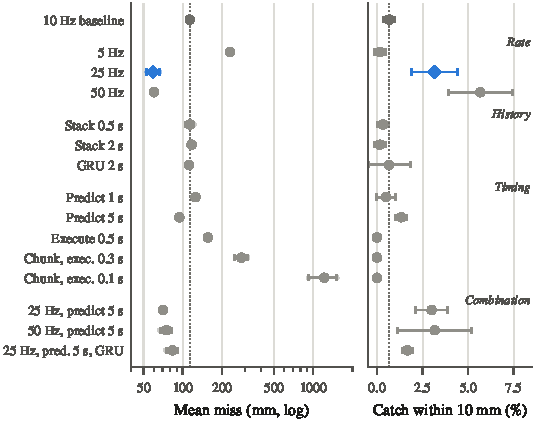
\includegraphics[width=\columnwidth]{fig_sweep}
\caption{Every swept configuration: mean over three seeds with sample s.d.; small dots are the individual seeds. The dotted lines mark the baseline. Only the rate family moves the miss substantially; the winner (diamond) is $25\,\mathrm{Hz}$ with the baseline timing.}
\label{fig:sweep}
\end{figure}

The rate prediction is confirmed. Halving the rate to $5\,\mathrm{Hz}$ doubles the miss to $230\,\mathrm{mm}$; $25\,\mathrm{Hz}$ lowers it to $59.1\,\mathrm{mm}$ with a $3.2\%$ catch rate, and $50\,\mathrm{Hz}$ gives $60.3\,\mathrm{mm}$ with $5.7\%$. The catch intervals of the two faster rates overlap and $25\,\mathrm{Hz}$ has the lower mean miss, so the ranking rule selects it. Beyond $25\,\mathrm{Hz}$ the miss does not fall further, even though the held-command change keeps shrinking (Fig.~\ref{fig:baseline}(a)).

History leaves the miss within $5\,\mathrm{mm}$ of the baseline at every level, as the analysis expected. The horizon prediction is refuted: predicting $1\,\mathrm{s}$ raises the miss to $125\,\mathrm{mm}$, while predicting $5\,\mathrm{s}$ and executing $1\,\mathrm{s}$ lowers it to $94\,\mathrm{mm}$. Open-loop growth along the chunk therefore did not identify a harmful horizon; a longer horizon appears to act as a smoother target. Shortening execution to $0.5\,\mathrm{s}$ raises the miss to $156\,\mathrm{mm}$, and the short-chunk prediction is confirmed: executing $0.3\,\mathrm{s}$ of a $0.5\,\mathrm{s}$ chunk misses by $281\,\mathrm{mm}$ and executing one $0.1\,\mathrm{s}$ step by $1219\,\mathrm{mm}$, a mean carried by misses above $2\,\mathrm{m}$.

The combination crosses $25$ and $50\,\mathrm{Hz}$ with the $5\,\mathrm{s}$ prediction, and adds the GRU to the $25\,\mathrm{Hz}$, $5\,\mathrm{s}$ cell. No combined cell beats the one-factor $25\,\mathrm{Hz}$ configuration, which is the winner: $25\,\mathrm{Hz}$, predict $2\,\mathrm{s}$, execute $1\,\mathrm{s}$, current frame, 1,000 demonstrations.

\subsection{From Baseline to Final Policy}
Fig.~\ref{fig:progression} follows the miss distribution through the study. The rate change moves the whole distribution: the pooled median falls from $100$ to $46\,\mathrm{mm}$ and the share within $50\,\mathrm{mm}$ rises from $19\%$ to $55\%$. Parking offsets move it again, to a median of $25\,\mathrm{mm}$, $91\%$ within $50\,\mathrm{mm}$, $9.8\%$ within $10\,\mathrm{mm}$ and a worst episode of $189\,\mathrm{mm}$. Command noise moves it the other way, to a median of $73\,\mathrm{mm}$. Table~\ref{tab:three} summarises the three retrained models.

\begin{figure}[t]
\centering
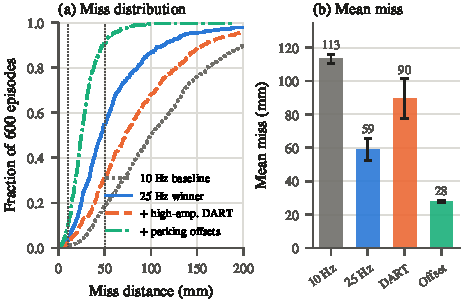
\includegraphics[width=\columnwidth]{fig_progression}
\caption{(a) Miss distribution of the four key models, pooling three seeds and 200 scenes; dotted lines at $10$ and $50\,\mathrm{mm}$. The axis ends at $200\,\mathrm{mm}$; the largest misses are $489$, $438$, $1042$ and $189\,\mathrm{mm}$. (b) Mean miss with the s.d. over seeds. DART and offset are the winner retrained on the 2,000-episode sets.}
\label{fig:progression}
\end{figure}

\begin{table}[t]
\centering
\caption{The ablation winner and the two retrains. Catch and miss: mean and sample s.d. over three seeds. Along and Side are the correction coefficients of Section~\ref{sec:eval} (1: arm absorbs the parking error).}
\label{tab:three}
\footnotesize
\setlength{\tabcolsep}{4pt}
\begin{tabular}{lcccc}
\toprule
Model & Catch (\%) & Miss (mm) & Along & Side \\
\midrule
Winner & $3.2\pm 1.3$ & $59.1\pm 6.8$ & $0.62\pm 0.04$ & $-0.23\pm 0.07$ \\
Command noise & $2.3\pm 1.8$ & $89.5\pm 11.8$ & $0.62\pm 0.13$ & $0.33\pm 0.13$ \\
Parking offset & $\mathbf{9.8\pm 2.0}$ & $\mathbf{27.9\pm 0.7}$ & $0.45\pm 0.02$ & $\mathbf{1.00\pm 0.05}$ \\
\bottomrule
\end{tabular}
\end{table}

\subsection{The Error Is a Parking Error}
\label{sec:parking}
Figs.~\ref{fig:transfer} and~\ref{fig:remaining} use a re-run of the same twelve checkpoints (baseline, winner and the two retrains, three seeds each) on the same 200 scenes, which records the per-episode geometry; its model means agree with Tables~\ref{tab:sweep} and~\ref{tab:three} to within $0.5\,\mathrm{mm}$.

For the baseline and the winner, the miss is almost entirely a parking error. At the closest approach the baseline's base sits a median $85\,\mathrm{mm}$ from the expert's, and the winner's $41\,\mathrm{mm}$ (Fig.~\ref{fig:remaining}(a)). Episode by episode, the miss tracks the magnitude of that parking error (correlation $0.94$ and $0.92$), and at a given parking error the two models miss by the same amount: their curves in Fig.~\ref{fig:remaining}(b) coincide. The faster rate does not make the arm more accurate; it parks the base twice as close, and the miss halves with it. A linear fit on the sideways parking error alone accounts for $89\%$ of the baseline's mean squared miss and $82\%$ of the winner's (Fig.~\ref{fig:remaining}(d)).

The winner follows the expert's route closely while driving, with a median offset of $13\,\mathrm{mm}$ in mid-route, and stops a median $10\,\mathrm{mm}$ ahead of the expert, consistent with braking later than the expert would in the same state (Fig.~\ref{fig:driving}).

\begin{figure}[t]
\centering
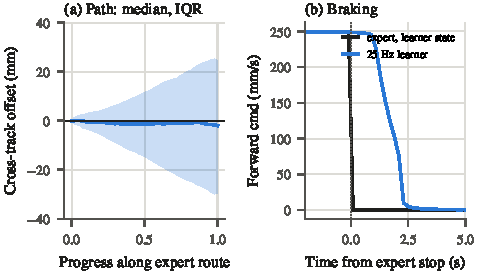
\includegraphics[width=\columnwidth]{fig_driving}
\caption{How the $25\,\mathrm{Hz}$ winner drives, 600 episodes. (a) Cross-track offset from the expert path against route progress: median and interquartile band. (b) Median forward command aligned to the expert's stop; the expert curve is queried in the learner's state. On the 379 rollouts that stop, the learner brakes a median $1.9\,\mathrm{s}$ later (quartiles $0.8$ and $3.3\,\mathrm{s}$).}
\label{fig:driving}
\end{figure}

What matters is how that parking error reaches the hand (Fig.~\ref{fig:transfer}(a)). Along the route the arm absorbs most of it, with a correction coefficient of $0.62$. Sideways it absorbs none: the coefficient is $-0.23$, so the hand misses by more than the base is off. The winner's median absolute hand miss is $41\,\mathrm{mm}$ sideways against $11\,\mathrm{mm}$ along the route and $9\,\mathrm{mm}$ vertically (Fig.~\ref{fig:remaining}(c)). Combined with the hand-off probe, in which the same arm catches once the expert has parked, this places the error in the base-to-arm hand-over. The demonstrations only ever show the arm reaching from the expert's exact parking point, so the arm never learned to reach from anywhere else.

\begin{figure*}[t]
\centering
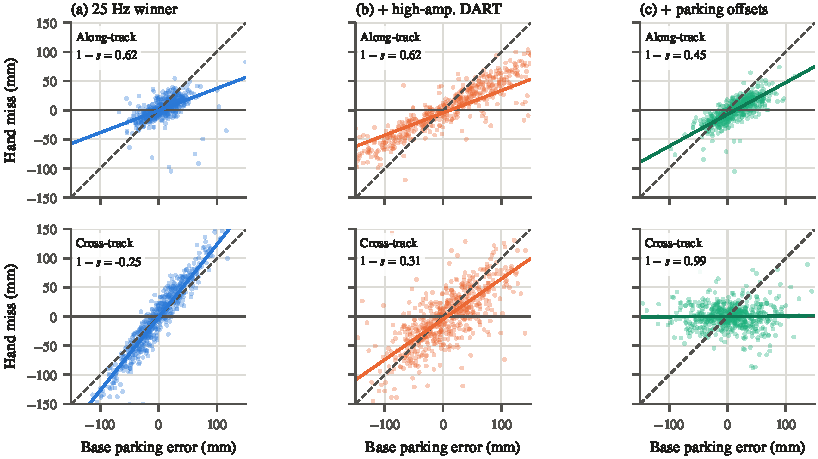
\includegraphics[width=\textwidth]{fig_transfer}
\caption{Hand miss against base parking error at the closest approach, in the expert's route frame, 600 episodes per model. Dashed: $y=x$, parking error passes straight to the hand. Horizontal line: $y=0$, the arm fully absorbs it. The solid line is the least-squares fit; its slope $s$ gives the correction coefficient $1-s$. (a) The winner corrects along the route but not sideways. (b) High-amplitude DART noise parks the base further off and still does not correct sideways. (c) Parking-offset demonstrations make the sideways fit flat: the arm absorbs sideways parking error, and along-track error is what passes through.}
\label{fig:transfer}
\end{figure*}

\begin{figure*}[t]
\centering
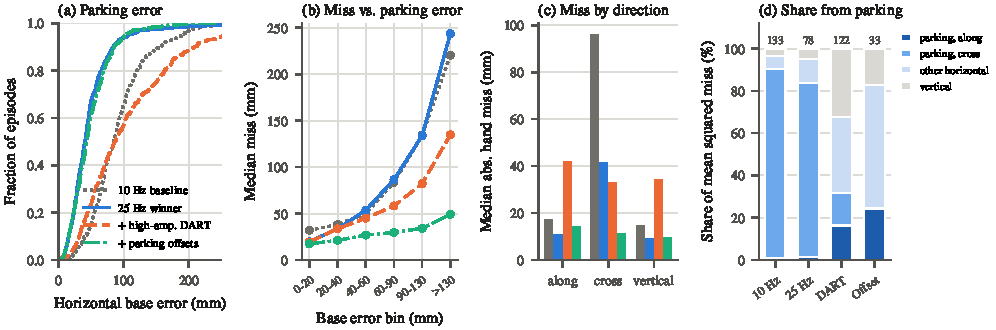
\includegraphics[width=\textwidth]{fig_remaining}
\caption{Where the error is, 600 episodes per model (legend in (a); colours as in all figures). (a) Horizontal base error at the closest approach. (b) Median miss in bins of base error, for bins with at least 10 episodes; the baseline and winner curves coincide. (c) Median absolute hand miss along the route, across it and vertically. (d) Mean squared 3-D miss split into the part a per-axis linear fit on the base error explains (``parking''), the rest of the horizontal miss, and the vertical miss; the RMS miss in mm is printed above each bar.}
\label{fig:remaining}
\end{figure*}

\subsection{High-Amplitude DART Fails}
\label{sec:dart}
DART~\cite{laskey2017} injects noise into the expert's executed commands so that demonstrations visit the states a learner would drift into, while the clean expert command is stored as the label. Following its recipe, we sized the noise to the learner's own error. On 50 rollouts of the winner the expert was queried at every tick in the learner's state, and an Ornstein--Uhlenbeck process was fitted to the learner-minus-expert command on each of the 18 channels. The fitted wheel standard deviation is $1.67\,\mathrm{rad/s}$ with a correlation time of $1.0$--$1.4\,\mathrm{s}$; arm position and velocity references have standard deviations of $0.095\,\mathrm{rad}$ and $0.031\,\mathrm{rad/s}$ on average.

Fig.~\ref{fig:dart} shows why that noise is unusable. Its RMS is $87\%$ of the clean wheel command and $55\%$ of the arm velocity command (Fig.~\ref{fig:dart}(b)), so the executed command bears little relation to the label (Fig.~\ref{fig:dart}(a)). Because the noise is correlated over about a second, the base integrates it into a random walk: in the example scene the expert ends more than a metre from its route (Fig.~\ref{fig:dart}(c)), and over the 1,000 demonstrations the median base distance from the clean expert at its catch time is $1.17\,\mathrm{m}$ (Fig.~\ref{fig:dart}(d)). The expert catches none of these episodes and misses by $1133\,\mathrm{mm}$ on average. The added half of the training set therefore shows states about thirty times further from the expert than the winner's typical $40\,\mathrm{mm}$ parking error, labelled with commands that do not lead to a catch from those states.

\begin{figure*}[t]
\centering
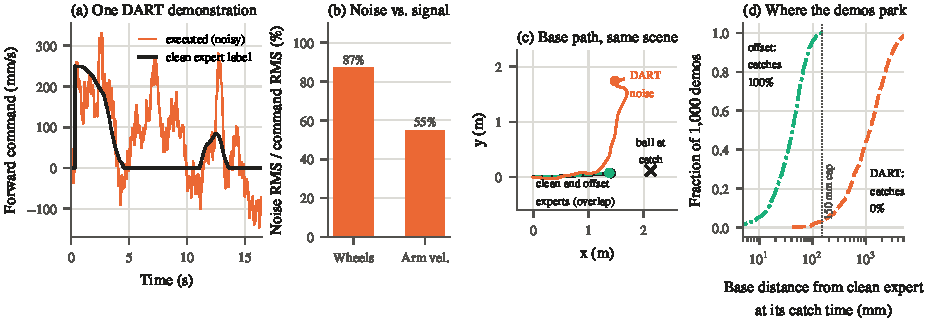
\includegraphics[width=\textwidth]{fig_dart_demos}
\caption{The high-amplitude DART demonstrations. (a) Forward wheel command in one demonstration: the stored clean label and the noisy command actually executed. (b) RMS of the injected noise relative to the RMS of the clean command, over all 1,000 demonstrations. (c) Base path in the same scene for the clean expert, the parking-offset expert and the noisy expert; dots mark the base at the clean expert's catch time. (d) Distance of the base from the clean expert's base at that time, over the 1,000 demonstrations of each extension. Offsets are capped at $150\,\mathrm{mm}$ and the offset expert still catches every ball; the noisy expert is a median $1.17\,\mathrm{m}$ away and catches none.}
\label{fig:dart}
\end{figure*}

The policy trained on this set is worse than the winner on every summary: mean miss $89.5\,\mathrm{mm}$, median $73\,\mathrm{mm}$, $32\%$ within $50\,\mathrm{mm}$. Its median parking error doubles, from $40$ to $86\,\mathrm{mm}$ (Fig.~\ref{fig:remaining}(a)), and the reach degrades as well: the median vertical miss rises from $9$ to $35\,\mathrm{mm}$ and the along-track miss from $11$ to $41\,\mathrm{mm}$ (Fig.~\ref{fig:remaining}(c)). The sideways correction coefficient improves from $-0.23$ to $0.33$, but the base is now further off in every direction (Fig.~\ref{fig:transfer}(b)). The fitted noise also discards structure in the learner's error: the wheel errors have a mean of $0.23$--$0.30\,\mathrm{rad/s}$, which the zero-mean process replaces with symmetric drift. Noise matched in variance and correlation time to a policy that is itself far from the expert produces demonstrations of failure, not of recovery.

\subsection{Parking Offsets and the Error That Remains}
The parking-offset set targets the hand-over directly. It perturbs only where the expert parks, by a median of $42\,\mathrm{mm}$, close to the winner's own $40\,\mathrm{mm}$ parking error, and the expert still catches every ball from there (Fig.~\ref{fig:dart}(d)). The arm thus sees demonstrations of reaching from realistically wrong base positions.

The retrained policy does not park better: its median base error is $44\,\mathrm{mm}$, the same distribution as the winner's (Fig.~\ref{fig:remaining}(a)). Its arm, however, now absorbs sideways parking error completely, with a correction coefficient of $1.00\pm0.05$ (Fig.~\ref{fig:transfer}(c)), and the median sideways hand miss falls from $41$ to $12\,\mathrm{mm}$. The share of the squared miss that sideways parking explains drops from $82\%$ to zero (Fig.~\ref{fig:remaining}(d)). The miss is lower at every level of parking error, and the penalty for a large one almost disappears: for episodes parked more than $130\,\mathrm{mm}$ off, the median miss is $49\,\mathrm{mm}$ against the winner's $244\,\mathrm{mm}$ (Fig.~\ref{fig:remaining}(b)). The mean miss is $27.9\,\mathrm{mm}$, the seed spread shrinks to $0.7\,\mathrm{mm}$, and the catch rate triples to $9.8\%$.

The error that remains is smaller and spread across directions: median absolute misses of $14\,\mathrm{mm}$ along the route, $12\,\mathrm{mm}$ across it and $10\,\mathrm{mm}$ vertically (Fig.~\ref{fig:remaining}(c)). Parking is still its largest attributable part. The along-track correction coefficient drops from $0.62$ to $0.45$, so about half of the along-track base error now passes into the hand, and the base still stops a median $19\,\mathrm{mm}$ ahead of the expert. That along-track term explains $58\%$ of the along-track miss and $24\%$ of the squared 3-D miss, the largest single component in Fig.~\ref{fig:remaining}(d), and the median miss still doubles across the parking-error bins, from $17\,\mathrm{mm}$ below $20\,\mathrm{mm}$ to $34\,\mathrm{mm}$ at $90$--$130\,\mathrm{mm}$. The remaining $58\%$ of horizontal error is not linearly tied to base position, and $17\%$ is vertical. Reaching the $10\,\mathrm{mm}$ radius reliably therefore needs better along-track parking, in particular braking on time, or offset demonstrations with more along-track spread than the $20\,\mathrm{mm}$ used here, together with a closer look at the residual not explained by base position.

\subsection{Cost}
The $10\,\mathrm{Hz}$ network has $7.4\times 10^{5}$ parameters and trains in $92\,\mathrm{s}$. The $25\,\mathrm{Hz}$ winner predicts 50 steps rather than 20, has $1.02\times 10^{6}$ parameters and trains in $193\,\mathrm{s}$; the $50\,\mathrm{Hz}$ network predicts 100 steps, has $1.48\times 10^{6}$ parameters and trains in $199\,\mathrm{s}$. The $10\,\mathrm{Hz}$ GRU has $8.7\times 10^{5}$ parameters and trains in $432\,\mathrm{s}$. The two $2{,}000$-episode retrains take $116$ and $119\,\mathrm{s}$. These are mean wall-clock training times over three seeds; closed-loop inference latency was not measured.

\section{Discussion and Limitations}
\subsection{What the Evidence Supports}
The baseline diagnosis was right about where the error was and partly right about what would fix it. The arm already catches from the expert's parking point, and the error accumulates while the base drives and parks. Raising the rate shortens the hold on a command that changes quickly while driving, halves the parking error, and through it halves the miss; at equal parking error the $10$ and $25\,\mathrm{Hz}$ policies miss by the same amount, so the rate does not teach the arm to reach from a misplaced base. Two of the three threshold-crossing predictions held (rate and short chunk), and the horizon prediction failed: open-loop error growth along a chunk was not a good guide to the closed-loop effect of the horizon.

The two extensions test the same idea, adding off-expert states to the data, in different ways. High-amplitude command noise sized to the learner's error drives the expert so far that it never catches; it adds unrecoverable states and raises the miss. Parking offsets of the size the learner actually makes keep the expert successful and teach exactly the missing skill, sideways base-to-arm correction. DART sets the noise level from the learner's error~\cite{laskey2017}, which assumes that error is small enough for the expert to still succeed under it. Here the learner's closed-loop command error is too large for that, and the recipe produces demonstrations of failure.

\subsection{Limits of the Perturbation Comparison}
Half of the original episodes already carry low-amplitude torque noise, which is a different perturbation from the high-amplitude command noise. Each extension doubles the training set, so comparing either against the winner mixes the perturbation with extra data; the comparison between the two extensions does not, since they share scenes and size. The command noise was not tuned in amplitude. A smaller scale might help, but it would no longer match the learner's error, which is the premise of the method.

\subsection{Validity and Remaining Gaps}
The factor sweep changes one setting at a time; only the combination stage changes families together. Holding chunk durations fixed in seconds means a faster policy also predicts more steps, so rate is not a change of clock alone. Inputs are noise-free simulated state, there is no grasp, and there is no hardware trial. Observation noise, actuation latency and trajectories outside the training generator were not measured. The 200 evaluation scenes ranked the sweep, so the winner has not been confirmed on a list withheld from the ranking. Every quoted mean includes the long tail.

\subsection{Future Work}
A scene list frozen before ranking, more training seeds, observation noise and a hardware trial would test whether the order in Table~\ref{tab:sweep} survives. On the method side, the analysis points at the along-track stop: offset demonstrations with wider along-track spread, or a policy that brakes on time, address the error that remains. None of these tests is assigned an expected gain.

\section{Conclusion}
The baseline's arm catches once the expert has parked; its error comes from driving and parking the base. Raising the policy rate from $10$ to $25\,\mathrm{Hz}$, as the pre-registered analysis predicted, halves the parking error and with it the mean miss, to $59\,\mathrm{mm}$, and raises the $10\,\mathrm{mm}$ catch rate from $0.7\%$ to $3.2\%$; history, a shorter prediction and a shorter execution window do not help, and a half-second chunk makes the miss several times larger. The winner's remaining error is a parking error that the arm does not correct sideways. High-amplitude DART noise matched to the winner's command error pushes the expert a metre off course, produces no successful demonstrations, and raises the miss to $90\,\mathrm{mm}$. Demonstrations from deliberately offset parking points lower it to $28\,\mathrm{mm}$, with $91\%$ of episodes within $50\,\mathrm{mm}$, by making the arm absorb sideways parking error. Along-track parking error is the largest attributable part of what remains. The study uses simulated state, a flat network and no grasp.

\begin{thebibliography}{1}
\bibitem{pomerleau1991}
D.~A. Pomerleau, ``Efficient training of artificial neural networks for autonomous navigation,'' \emph{Neural Comput.}, vol.~3, no.~1, pp.~88--97, 1991.
\bibitem{ross2011}
S.~Ross, G.~J. Gordon, and J.~A. Bagnell, ``A reduction of imitation learning and structured prediction to no-regret online learning,'' in \emph{Proc. 14th Int. Conf. Artif. Intell. Statist.}, 2011, pp.~627--635.
\bibitem{laskey2017}
M.~Laskey, J.~Lee, R.~Fox, A.~Dragan, and K.~Goldberg, ``{DART}: Noise injection for robust imitation learning,'' in \emph{Proc. 1st Conf. Robot Learn.}, 2017, pp.~143--156.
\bibitem{pybullet}
E.~Coumans and Y.~Bai, ``PyBullet, a Python module for physics simulation for games, robotics and machine learning,'' 2016. [Online]. Available: \url{http://pybullet.org}
\bibitem{pinocchio}
J.~Carpentier \emph{et al.}, ``The {P}inocchio {C}++ library: A fast and flexible implementation of rigid body dynamics algorithms and their analytical derivatives,'' in \emph{Proc. IEEE/SICE Int. Symp. Syst. Integr.}, 2019, pp.~614--619.
\end{thebibliography}

% Separate statement, up to one additional page under the assignment brief.
\clearpage
\section*{Contribution Statement}
% BLANK: group members must supply their actual contributions.

\end{document}
